\documentclass{article}

% NeurIPS-compatible packages
\usepackage[final]{neurips_2024}   % swap 'final' for 'preprint' if needed
\usepackage[utf8]{inputenc}
\usepackage[T1]{fontenc}
\usepackage{hyperref}
\usepackage{url}
\usepackage{booktabs}
\usepackage{amsfonts}
\usepackage{amsmath}
\usepackage{amssymb}
\usepackage{nicefrac}
\usepackage{microtype}
\usepackage{xcolor}
\usepackage{graphicx}
\usepackage{caption}
\usepackage{subcaption}
\usepackage{multirow}
\usepackage{array}
\usepackage{enumitem}

% ─────────────────────────────────────────────────────────────
\title{Spectral Dynamics of Attention Under Cognitive Load:\\
       Low-Rank Dissipation of Multi-Head Attention\\
       Across Bloom's Taxonomy}

\author{%
  Vedant Maheshwari \\
  \texttt{vedant.maheshwari@example.com}
}

\begin{document}
\maketitle

% ═══════════════════════════════════════════════════════════════
\begin{abstract}
We treat the self-attention matrix as an evolving linear operator in a
dynamical system and use Singular Value Decomposition~(SVD) to perform
controlled rank ablation on Phi-2~(2.7B) during autoregressive generation.
Intervening simultaneously on layers~15--20 and~31 with top-$k$ truncation
($k\!\in\!\{1,\ldots,5\}$) across 42 chain-of-thought prompts graded along
Bloom's Taxonomy of Learning~(BTL), we reveal three structural phenomena.
\textbf{(i) The depth gradient:} intermediate reasoning layers (15--20) operate
as BTL-invariant, strongly dissipative rank-2 funnels
($r_{\text{eff}}\!\approx\!2.6$--$3.7$, energy ${\geq}67\%$ at $k\!=\!1$),
while the final layer~(31) expands to $r_{\text{eff}}\!\approx\!5.2$ and retains
only $\sim\!50\%$ energy at $k\!=\!1$, scaling explicitly with sequence context.
\textbf{(ii) The W-shape anomaly:} KL divergence is non-monotonic in cognitive
level; procedural Understanding prompts are the most sensitive ($D_\text{KL}\!=\!0.283$)
while open-ended Evaluating prompts are the most robust~($D_\text{KL}\!=\!0.186$),
contradicting the intuitive assumption that higher cognitive levels are more fragile.
\textbf{(iii) The paraphrasing phenomenon:} SVD truncation never produces incoherent
output; instead it displaces the generation into one of five qualitatively
distinct behavioural archetypes (formulaic immunity, template preservation,
lexical substitution, discourse framework shift, interrogative collapse, and
contextual genericization) determined by task type.
A zero correlation $(\rho\!=\!{-}0.006)$ between spectral rank and
autoregressive text divergence confirms that generation behaves as a
chaotic dynamical system, where trajectory divergence is driven by
compounding distributional shifts, not by the initial perturbation magnitude.
\end{abstract}

% ═══════════════════════════════════════════════════════════════
\section{Introduction}
\label{sec:intro}

Self-attention \citep{vaswani2017attention} is the dominant information-routing
mechanism in modern language models.  Despite its ubiquity, fundamental questions
remain about how much of its full-rank representational capacity is functionally
used during inference.  Prior theoretical work shows that pure self-attention without
residual connections loses rank \emph{doubly exponentially} with depth
\citep{dong2021attention}, suggesting that real-world MHA layers operate far below
their nominal rank budget.  Yet, it is unclear whether this low-rank behaviour is
uniform across layers, uniform across task types, or exploitable for inference
compression without quality loss.

We attack this question empirically through \emph{surgical rank ablation}.
Using Singular Value Decomposition, we intercept the post-softmax attention
matrix $A$ inside each targeted layer, retain only the top-$k$ singular components,
and inject the rank-$k$ approximation back into the computation graph for the
remainder of that forward pass.  No weights are modified; the model is the
stock Phi-2 model with eager attention.

Setting the stage for a principled evaluation, we ground our prompts in
Bloom's Taxonomy of Learning~\citep{bloom1956taxonomy}, a six-level cognitive
hierarchy spanning Remembering, Understanding, Applying, Analyzing, Evaluating,
and Creating.  This taxonomy lets us ask: \emph{does the rank needed to preserve
generation quality scale with cognitive complexity?}

Our answer is nuanced and empirically rich.  We show that:
\begin{itemize}[leftmargin=1.5em, itemsep=0pt]
  \item The rank requirements of intermediate layers are \emph{task-invariant}
        and naturally low ($r_{\text{eff}}\!\approx\!2$--3), but Layer~31 is
        \emph{task-sensitive} and dramatically higher ($r_{\text{eff}}\!\approx\!5.2$).
  \item KL divergence follows a W-shaped, non-monotonic pattern across BTL levels,
        which we explain by the structure of attentional dominance, not cognitive
        difficulty per se.
  \item Generated text under SVD truncation does not degrade to nonsense;
        it transitions through identifiable stylistic archetypes, revealing
        what information each singular mode encodes.
  \item Autoregressive text divergence is chaotic: it cannot be predicted from
        the magnitude of the initial spectral perturbation.
\end{itemize}

% ═══════════════════════════════════════════════════════════════
\section{Related Work}
\label{sec:related}

\paragraph{Low-rank attention.}
Linformer \citep{wang2020linformer} projects keys and values to a fixed low-rank
space, demonstrating that $O(n)$ attention is achievable with minimal quality loss
on classification tasks.  Our work operates orthogonally: we ablate the \emph{output}
attention matrix during inference, not the projection matrices, and evaluate effects
on long-form autoregressive generation rather than classification.

\paragraph{Rank collapse theory.}
\citet{dong2021attention} prove that stacking pure self-attention collapses token
representations to rank 1 doubly exponentially unless mitigated by MLPs and
residual connections.  Our empirical findings confirm this collapse in intermediate
layers of Phi-2 and reveal that the final layer resists it---a complementary
observation not predicted by the purely feed-forward theoretical setting.

\paragraph{Low-rank adaptation.}
LoRA \citep{hu2021lora} rewrites weight updates as low-rank matrix products,
demonstrating that fine-tuning can be performed in a dramatically compressed
parameter space.  Our work is distinct: we target the \emph{activation} matrix
at inference time and measure cognitive-load-dependent sensitivity, rather than
training efficiency.

\paragraph{Mechanistic interpretability.}
\citet{olsson2022incontext} identify ``induction heads'' that implement in-context
learning; \citet{wang2022interpretability} identify attention heads implementing
specific circuits.  Our spectral lens provides a complementary, holistic view:
rather than labelling heads by function, we characterise entire layers by their
intrinsic dimensionality and its relationship to task complexity.

% ═══════════════════════════════════════════════════════════════
\section{Background and Problem Formulation}
\label{sec:background}

\subsection{SVD Truncation of the Attention Operator}

Let $A \in \mathbb{R}^{Q \times K}$ be the causal post-softmax attention matrix
for a single head, where in the prefill stage $Q\!=\!K\!=\!N$ (sequence length).
We decompose $A$ as:
\begin{equation}
  A = U \Sigma V^\top, \qquad \Sigma = \mathrm{diag}(\sigma_1, \sigma_2, \ldots, \sigma_N),
  \quad \sigma_1 \geq \sigma_2 \geq \cdots \geq \sigma_N \geq 0.
\end{equation}
The rank-$k$ approximation retains only the $k$ largest singular triplets:
\begin{equation}
  A_k = U_k \Sigma_k V_k^\top = \sum_{i=1}^{k} \sigma_i \, u_i v_i^\top.
  \label{eq:truncation}
\end{equation}
We substitute $A_k$ for $A$ in the computation $A_k V_{\text{states}}$, where
$V_{\text{states}}$ are the value projections.  All other computations (projections,
residual stream, MLP blocks) are unmodified.

\subsection{Spectral Metrics}

We define a spectral probability distribution via normalised squared singular values:
\begin{equation}
  p_i = \frac{\sigma_i^2}{\sum_j \sigma_j^2}.
\end{equation}
From this we compute four metrics per head:
\begin{align}
  \text{Energy retained} &= E_{\text{ret}}(k) = \sum_{i=1}^{k} p_i \times 100\%, \\
  \text{Spectral entropy} &= H = -\sum_i p_i \ln p_i, \\
  \text{Effective rank}   &= r_{\text{eff}} = e^H, \\
  \text{Top-1 dominance}  &= d_1 = \sigma_1 / \sum_i \sigma_i.
\end{align}
$r_{\text{eff}}$ provides a continuous, entropy-weighted measure of matrix rank
\citep{roy2007effective} that is more informative than the integer rank because it
weights each mode by its functional contribution.

\subsection{Output Divergence Metrics}

For each prompt $p$, we measure three output-level divergence quantities under
rank-$k$ truncation:
\begin{align}
  D_\text{KL}(k) &= D_\text{KL}\!\left( \mathcal{P}_\text{base} \;\|\; \mathcal{P}_k \right)
    = \sum_v P_\text{base}(v) \ln \frac{P_\text{base}(v)}{P_k(v)+\epsilon}, \\
  \overline{|\Delta \ell|}(k) &= \frac{1}{|V|}\sum_v |L_\text{base}(v) - L_k(v)|, \\
  \text{Jaccard}(k) &= \frac{|W_\text{base} \cap W_k|}{|W_\text{base} \cup W_k|},
\end{align}
where $\mathcal{P}$ denotes next-token softmax distributions and $W$ is the bag of
generated word types.

% ═══════════════════════════════════════════════════════════════
\section{Experimental Setup}
\label{sec:setup}

\paragraph{Model.}
We use \texttt{microsoft/phi-2} (2.7B parameters, 32 transformer layers, 32 heads,
head dimension 80, MHA) loaded in \texttt{bfloat16} on CUDA with
\texttt{attn\_implementation=''eager''} to expose raw attention tensors.

\paragraph{Intervention.}
We implement a \texttt{MultiLayerSVDPatcher} context manager that monkey-patches
the \texttt{forward} method of each targeted layer's self-attention module.
The patch recomputes $Q, K, V$ projections, applies rotary embeddings, computes
softmax attention, applies Eq.~\eqref{eq:truncation} to each head independently,
and forwards the modified output through the dense projection.
KV caching is disabled to ensure truncation is applied at every autoregressive step.
Target layers: $\{15, 16, 17, 18, 19, 20, 31\}$; sweep: $k \in \{1, 2, 3, 4, 5\}$.

\paragraph{BTL evaluation suite.}
We design 42 chain-of-thought prompts, seven per BTL level, formatted as:
\begin{quote}
\small
\texttt{Instruct: Provide a detailed, step-by-step reasoning chain...\\
Request: \{prompt\}\\
Output: Let's think step by step. Step 1:}
\end{quote}
Topics span history, physics, engineering, ethics, literature, and design
(see Appendix~A for the full list).
Mean sequence length: 76 tokens (range: 67--87).
Generation: greedy decoding, 200 new tokens.

\paragraph{Spectral metadata collection.}
We capture the original (pre-truncation) attention tensor at prefill time
($Q_\text{len} = K_\text{len}$) for each layer, compute all four spectral metrics
per head, and average across heads.  This gives us per-layer, per-prompt,
per-$k$ spectral measurements for all 42$\times$5$\times$7 = 1,470 data points.

% ═══════════════════════════════════════════════════════════════
\section{Results I: Spectral Structure Across Layers}
\label{sec:spectral}

\subsection{The Depth Gradient}

Table~\ref{tab:spectral} reports the mean spectral metrics at $k=1$ averaged
across all 42 BTL prompts.  Three structural facts are immediately apparent.

\begin{table}[h]
\centering
\caption{Mean per-head spectral metrics at $k=1$, averaged over all 42 BTL prompts.
$r_\text{eff}$: effective rank; $H$: spectral entropy (bits); $E_\text{ret}$: energy
retained (\%); $d_1$: top-1 dominance; $\Delta\sigma$: spectral gap $\sigma_1-\sigma_2$;
$N_\text{sig}$: mean count of singular values $>1\%$ of $\sigma_1$.}
\label{tab:spectral}
\begin{tabular}{lcccccc}
\toprule
\textbf{Layer} & $r_\text{eff}$ & $H$ (bits) & $E_\text{ret}$ (\%) & $d_1$ & $\Delta\sigma$ & $N_\text{sig}$ \\
\midrule
L15 & 2.76 & 1.39 & 71.8 & 0.372 & 2.256 & 26.2 \\
L16 & 2.66 & 1.28 & 73.1 & 0.405 & 2.383 & 22.0 \\
L17 & 2.63 & 1.35 & 72.0 & 0.371 & 2.211 & 26.3 \\
L18 & 2.90 & 1.41 & 70.4 & 0.372 & 2.186 & 25.8 \\
L19 & 3.13 & 1.50 & 69.5 & 0.355 & 2.148 & 27.3 \\
L20 & 3.65 & 1.66 & 66.9 & 0.337 & 2.095 & 29.5 \\
\textbf{L31} & \textbf{5.17} & \textbf{2.01} & \textbf{50.1} & \textbf{0.313} & \textbf{1.055} & 25.3 \\
\bottomrule
\end{tabular}
\end{table}

\textbf{Layer 31 is spectrally unique.}
Compared to the intermediate block~(L15--20), Layer~31 has 1.8$\times$ higher
effective rank, 0.73~bits more spectral entropy, retains only half its energy at
$k=1$ (50\% vs.\ 67--73\%), and exhibits a much smaller spectral gap
(1.06~vs.\ 2.1--2.4)---meaning $\sigma_1$ and $\sigma_2$ compete rather than one
dominating.  The intermediate layers L15--L17 are the most dissipative
($r_\text{eff}\!\approx\!2.63$--$2.76$), with L18--L20 forming a gradual
transition upward.

\begin{figure}[h]
  \centering
  \begin{subfigure}{0.48\textwidth}
    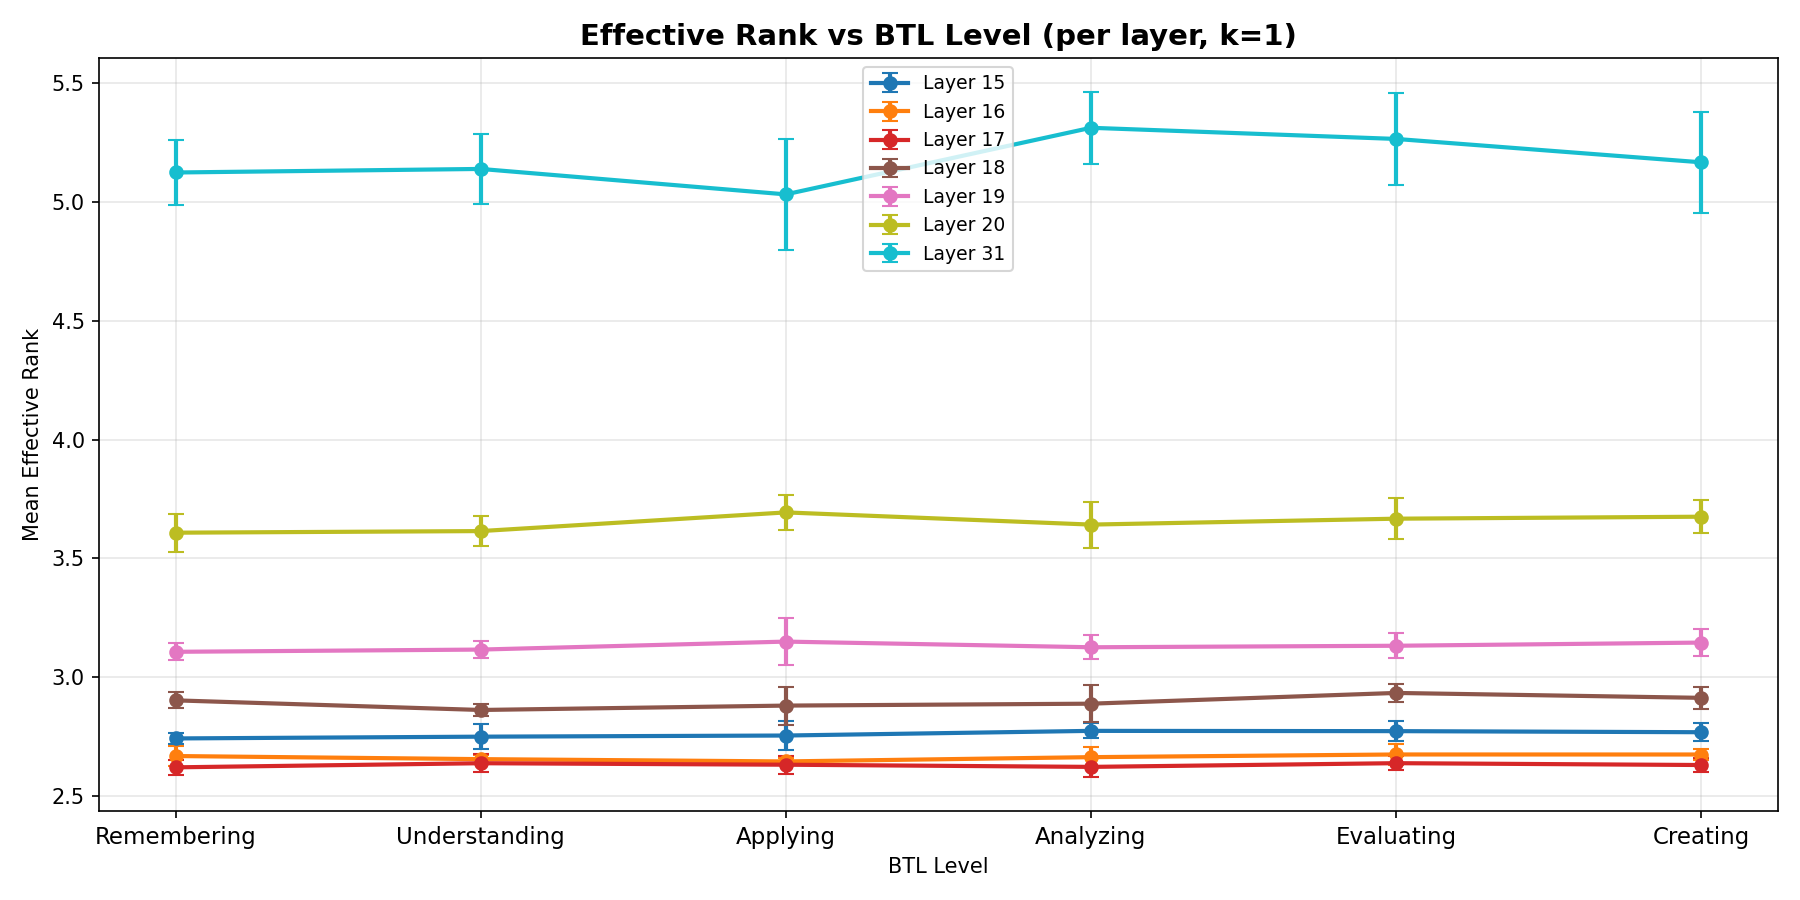
\includegraphics[width=\textwidth]{plots/eff_rank_vs_btl.png}
    \caption{Effective rank per layer and BTL level at $k=1$.
             Layer~31 (top curve) is uniformly higher; L15--L17 are flat.}
  \end{subfigure}
  \hfill
  \begin{subfigure}{0.48\textwidth}
    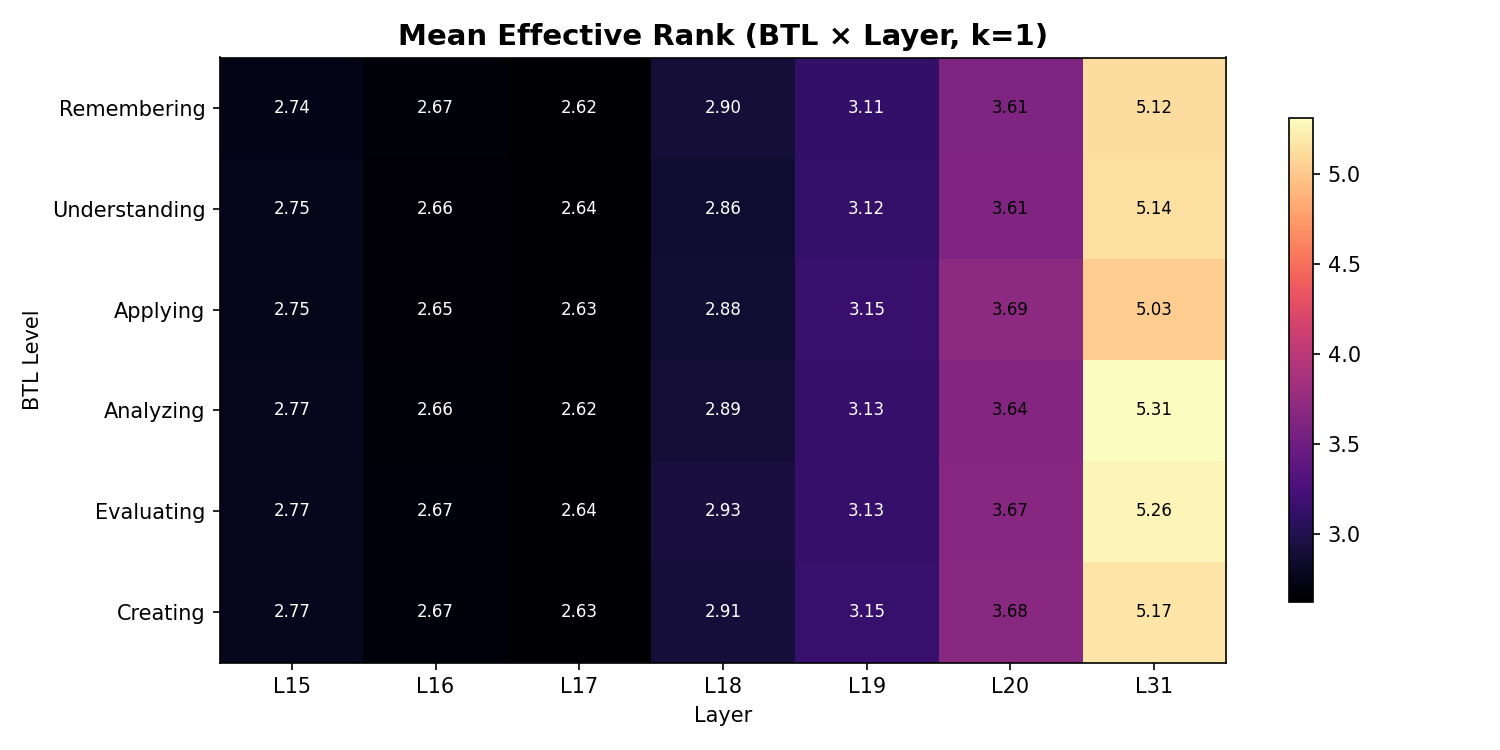
\includegraphics[width=\textwidth]{plots/heatmap_rank_btl_layer.png}
    \caption{Heatmap of BTL level $\times$ layer effective rank.
             BTL variation lives almost entirely in Layer~31.}
  \end{subfigure}
  \caption{Effective rank across layers and Bloom's Taxonomy levels.
           Intermediate layers are BTL-invariant; Layer~31 encodes task-level
           spectral variation.}
  \label{fig:rank}
\end{figure}

\textbf{BTL variation is confined to Layer~31.}
The heatmap in Figure~\ref{fig:rank}(b) shows that L15--L20 ranks are nearly
identical across all BTL levels ($r_\text{eff}$ range: 2.62--3.69 with
cross-BTL std~$\leq\!0.10$).  Layer~31 shows a wider spread:
Analyzing ($r_\text{eff}\!=\!5.31$) and Evaluating ($r_\text{eff}\!=\!5.26$)
rank highest; Applying ($r_\text{eff}\!=\!5.03$) ranks lowest.

\textbf{Effective rank scales with context length.}
A single 13-token control prompt yields $r_\text{eff}^{L31}\!=\!2.84$; the 42
BTL prompts at $\sim\!76$ tokens yield $r_\text{eff}^{L31}\!=\!5.17$---a
\textbf{1.8$\times$ increase} for a 5.8$\times$ increase in sequence length.
Figure~\ref{fig:seqlen} shows this relationship across prompts, with no confound
from BTL level (Pearson $r\!=\!0.06$ between sequence length and rank within
the 42-prompt set).

\begin{figure}[h]
  \centering
  \begin{subfigure}{0.48\textwidth}
    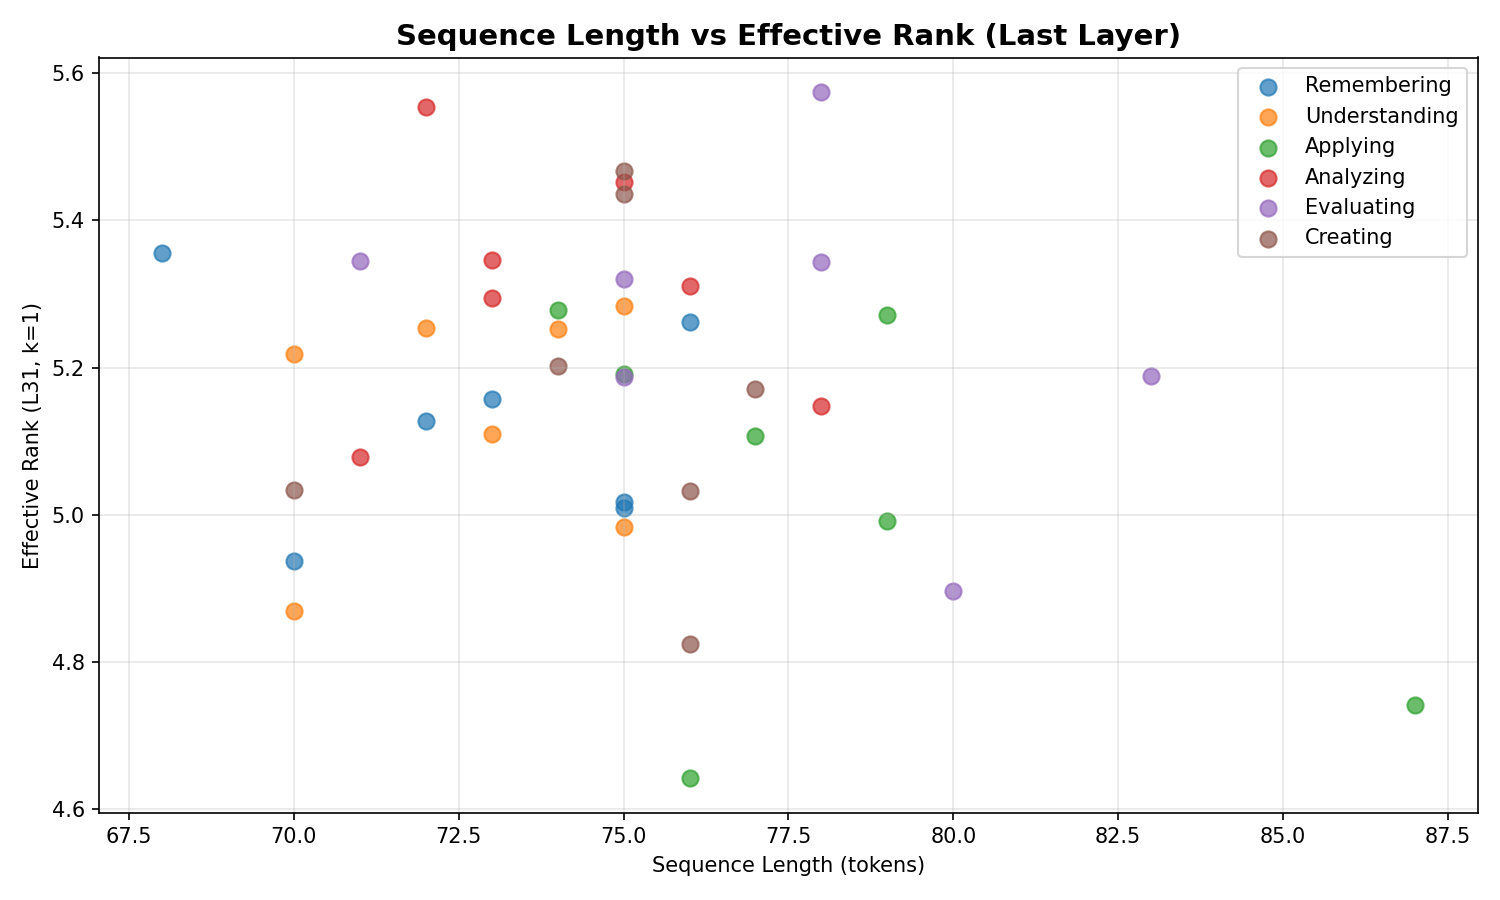
\includegraphics[width=\textwidth]{plots/seqlen_vs_rank.png}
    \caption{Effective rank at Layer~31 vs.\ sequence length.
             Each point is one BTL prompt; colours denote BTL level.}
  \end{subfigure}
  \hfill
  \begin{subfigure}{0.48\textwidth}
    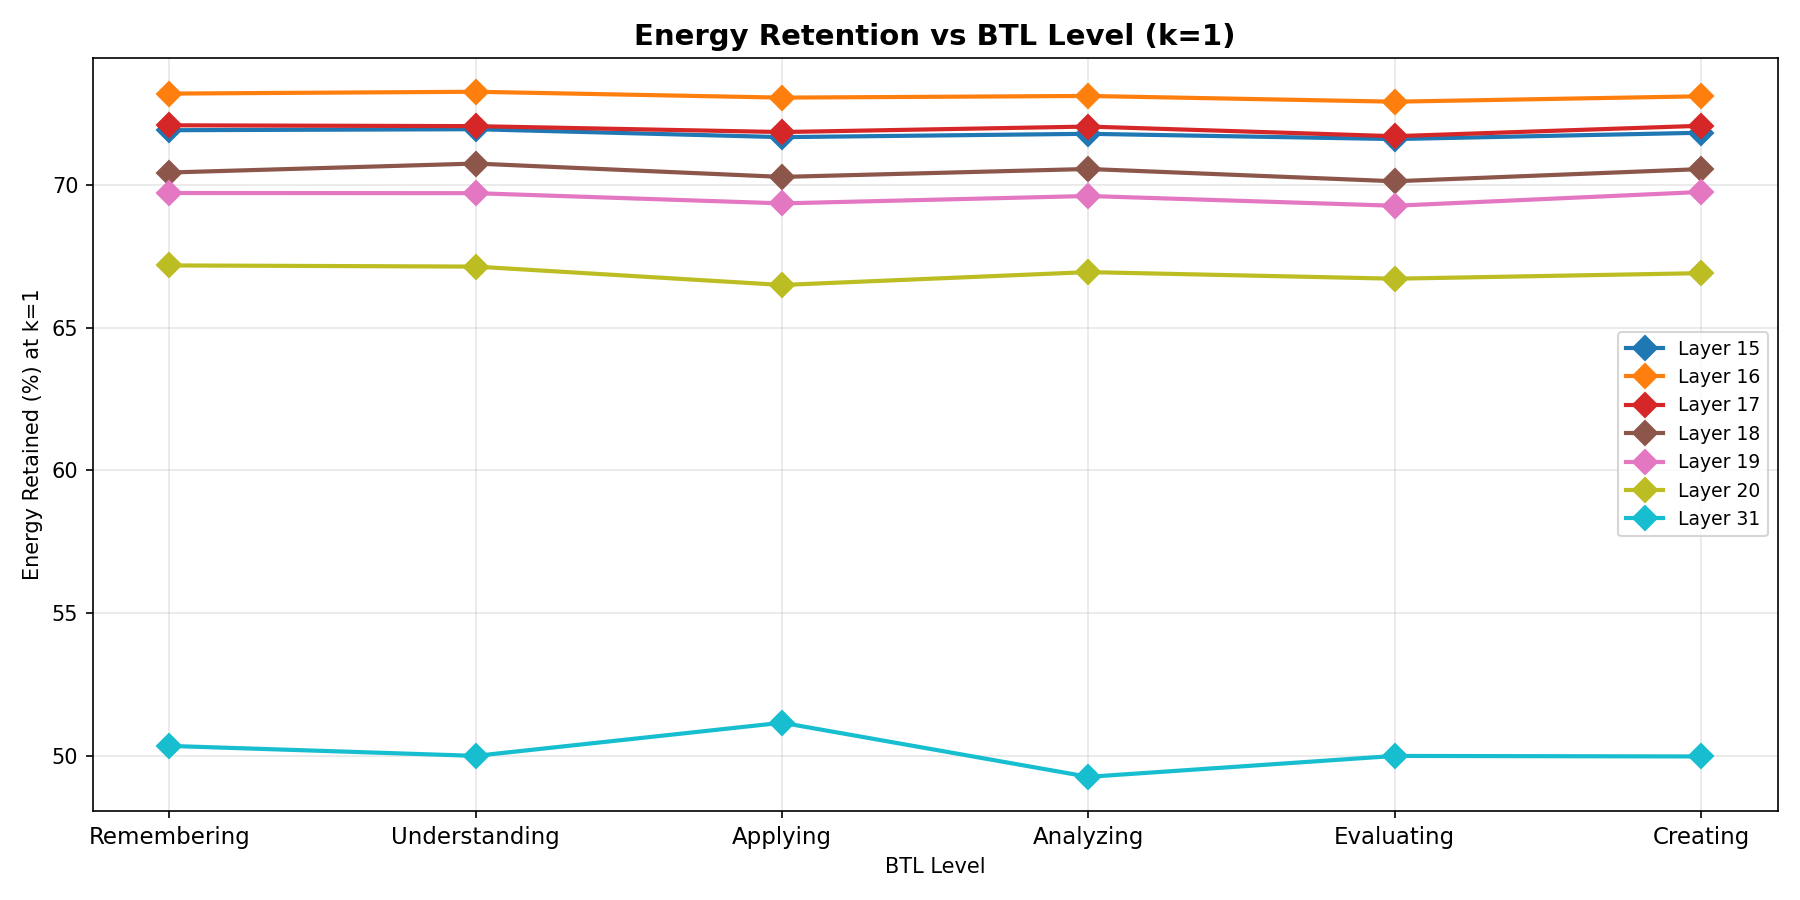
\includegraphics[width=\textwidth]{plots/energy_vs_btl.png}
    \caption{Energy retained at $k=1$ per layer.
             Layer~31 (bottom curve) retains only 50\%; L15--16 retain $\geq$73\%.}
  \end{subfigure}
  \caption{Context-length dependence and energy retention by layer.}
  \label{fig:seqlen}
\end{figure}

\subsection{Energy Convergence and the k=2 Sweet Spot}

Figure~\ref{fig:energy_k} shows mean energy retained as a function of $k$
per layer, measured on the single-prompt baseline (which isolates layer effects
without BTL confounds).

\begin{figure}[h]
  \centering
  \begin{subfigure}{0.48\textwidth}
    
\includegraphics[width=\textwidth]{../svd_multilayer_outputs/energy_vs_k_per_layer.png}
    \caption{Energy retained vs.\ $k$ per layer.
             L15--20 converge at $k\!=\!2$; L31 converges slowly through $k\!=\!5$.}
  \end{subfigure}
  \hfill
  \begin{subfigure}{0.48\textwidth}
    
\includegraphics[width=\textwidth]{../svd_multilayer_outputs/eff_rank_vs_k_per_layer.png}
    \caption{Effective rank vs.\ $k$: constant (property of original matrix).
             Note the L31 offset from all other layers.}
  \end{subfigure}
  \caption{Energy convergence and effective rank across truncation levels.
           $k\!=\!2$ is the compression sweet spot for L15--20;
           Layer~31 requires $k\!\geq\!5$ for comparable fidelity.}
  \label{fig:energy_k}
\end{figure}

Layers~15--20 jump from 75--78\% (at $k\!=\!1$) to $\geq\!98\%$ energy retained
at $k\!=\!2$---an $\sim\!23$ percentage-point gain for one additional mode.
Layer~31 climbs more gradually: 66\%$\to$85\%$\to$93\%$\to$95\%$\to$97.5\%
at $k\!=\!1$\dots5, never fully converging within the sweep.
This establishes that \textbf{$k\!=\!2$ is the practical compression threshold for
intermediate layers}, while \textbf{Layer~31 is the bottleneck for any attention
compression scheme}---it requires dedicated higher-rank budget.

% ═══════════════════════════════════════════════════════════════
\section{Results II: BTL Sensitivity and the W-Shape Anomaly}
\label{sec:btl}

\subsection{KL Divergence Across BTL Levels}

Table~\ref{tab:kl} reports mean KL divergence at each $k$ for all six BTL levels.

\begin{table}[h]
\centering
\caption{Mean KL divergence $D_\text{KL}$ (and std) at each truncation level $k$, per BTL level.
Rows sorted by $D_\text{KL}(k=1)$ descending.}
\label{tab:kl}
\begin{tabular}{lcccccc}
\toprule
\textbf{BTL Level} & $k\!=\!1$ & $k\!=\!2$ & $k\!=\!3$ & $k\!=\!4$ & $k\!=\!5$ \\
\midrule
Understanding & 0.283$_{\pm0.198}$ & 0.271$_{\pm0.170}$ & 0.206$_{\pm0.086}$ & 0.161$_{\pm0.088}$ & 0.092$_{\pm0.041}$ \\
Applying      & 0.264$_{\pm0.082}$ & 0.244$_{\pm0.073}$ & 0.209$_{\pm0.073}$ & 0.118$_{\pm0.037}$ & 0.072$_{\pm0.024}$ \\
Creating      & 0.234$_{\pm0.139}$ & 0.215$_{\pm0.113}$ & 0.182$_{\pm0.071}$ & 0.102$_{\pm0.020}$ & 0.068$_{\pm0.016}$ \\
Remembering   & 0.198$_{\pm0.042}$ & 0.174$_{\pm0.032}$ & 0.171$_{\pm0.043}$ & 0.107$_{\pm0.045}$ & 0.094$_{\pm0.052}$ \\
Analyzing     & 0.194$_{\pm0.042}$ & 0.193$_{\pm0.057}$ & 0.162$_{\pm0.059}$ & 0.108$_{\pm0.026}$ & 0.071$_{\pm0.023}$ \\
Evaluating    & \textbf{0.186}$_{\pm0.093}$ & \textbf{0.173}$_{\pm0.086}$ & \textbf{0.143}$_{\pm0.070}$ & \textbf{0.103}$_{\pm0.019}$ & \textbf{0.067}$_{\pm0.014}$ \\
\midrule
\textit{Mean all} & 0.227 & 0.212 & 0.179 & 0.117 & 0.077 \\
\bottomrule
\end{tabular}
\end{table}

\begin{figure}[h]
  \centering
  \begin{subfigure}{0.52\textwidth}
    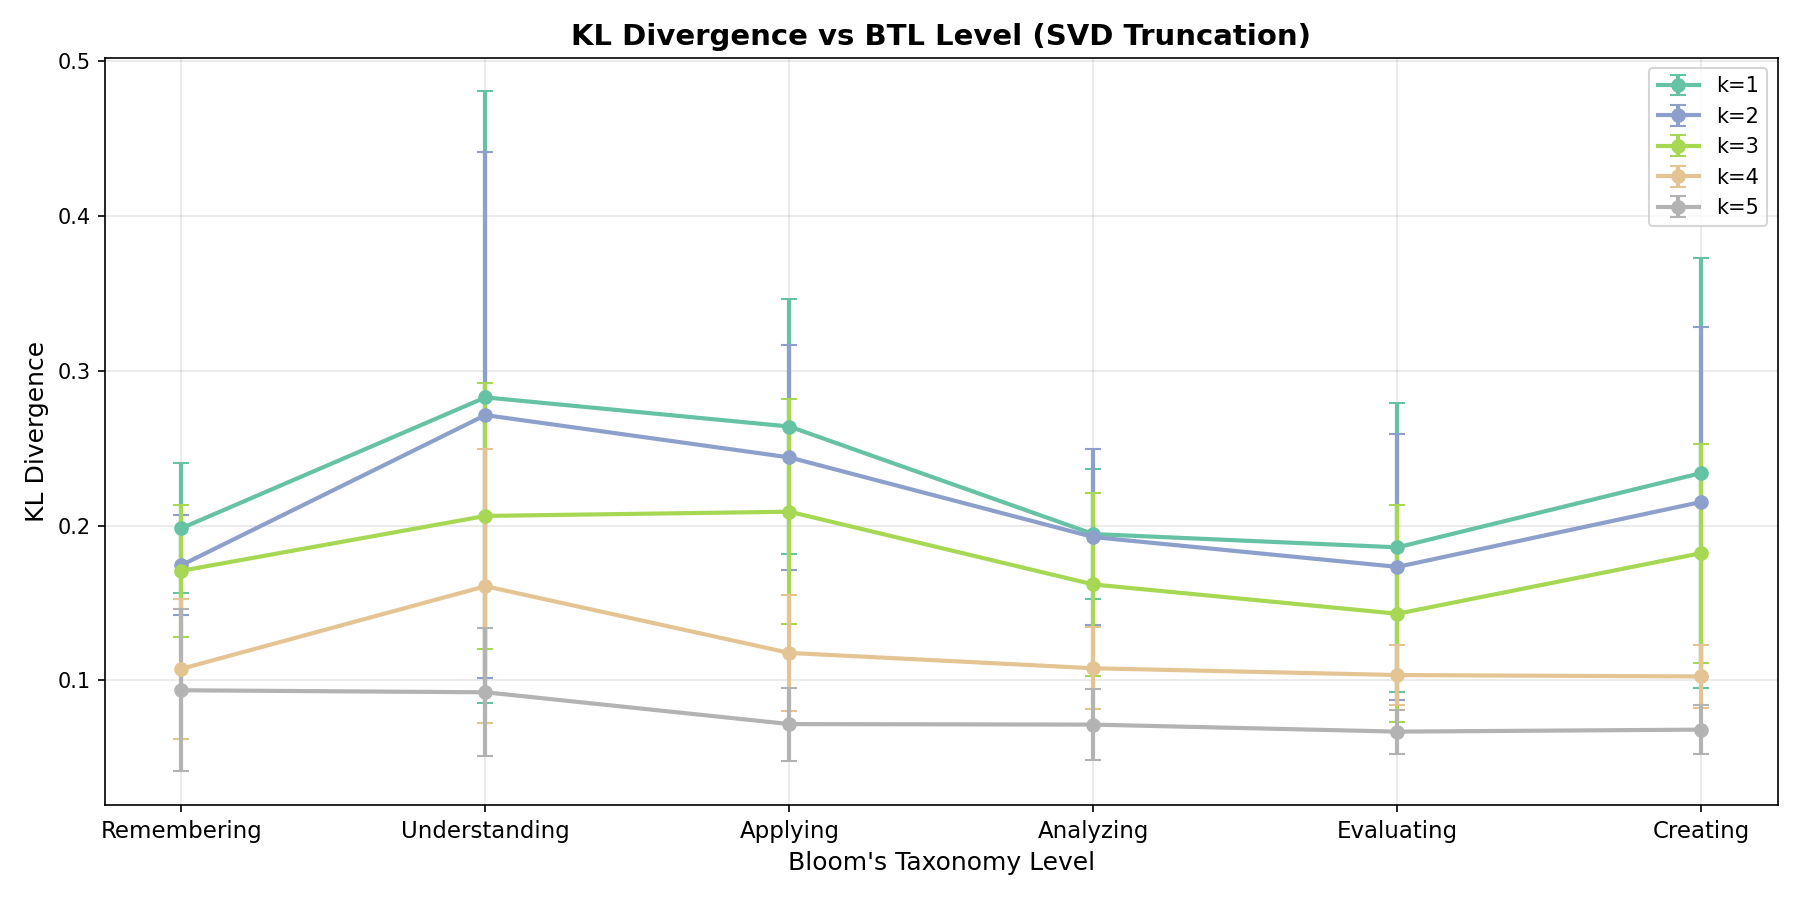
\includegraphics[width=\textwidth]{plots/kl_vs_btl.png}
    \caption{KL divergence per BTL level with error bars across $k$.
             Note the non-monotonic W-shape: Understanding peaks, Evaluating troughs.}
  \end{subfigure}
  \hfill
  \begin{subfigure}{0.44\textwidth}
    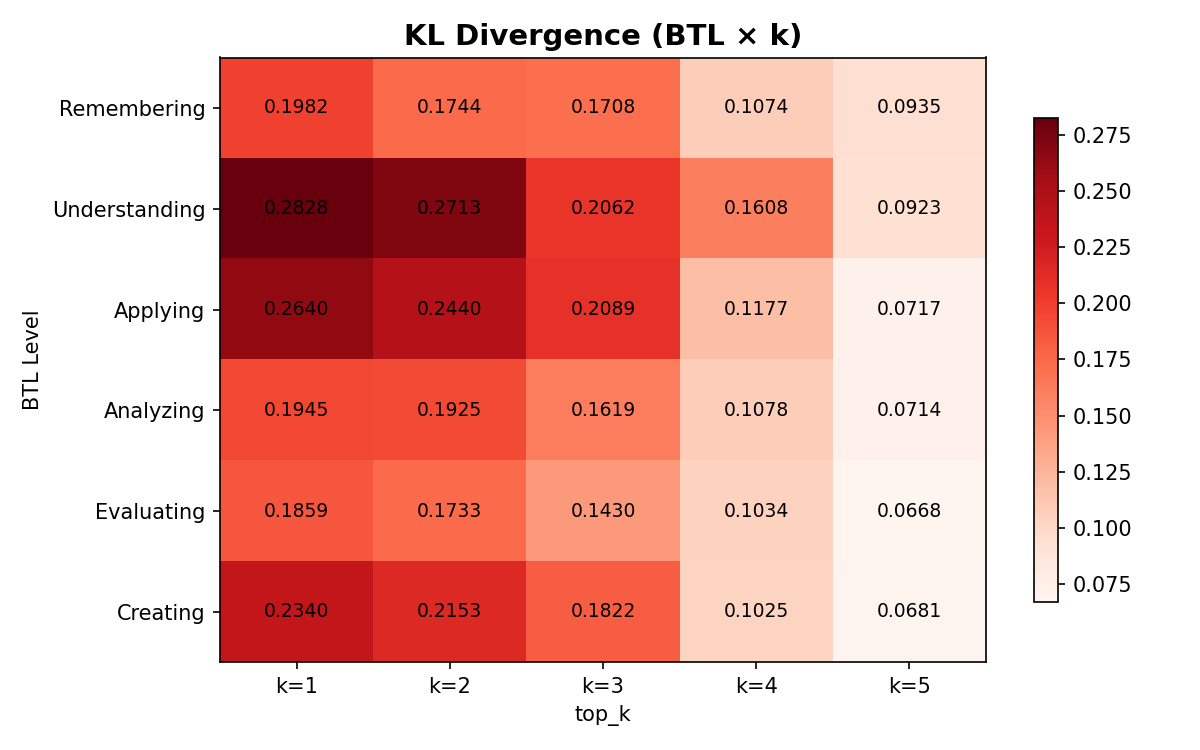
\includegraphics[width=\textwidth]{plots/heatmap_kl_btl_k.png}
    \caption{Heatmap: KL divergence (BTL level $\times$ k).  All levels converge
             smoothly; the W-shape ordering is preserved throughout.}
  \end{subfigure}
  \caption{KL divergence patterns across Bloom's Taxonomy and truncation rank.}
  \label{fig:kl}
\end{figure}

\subsection{The W-Shape: An Explanation}

The W-shape ordering (Understanding $>$ Applying $>$ Creating $\gg$ Remembering $\approx$
Analyzing $>$ Evaluating) contradicts the intuition that higher BTL levels are more
fragile.  We explain it via two mechanisms.

\textbf{Distributional spread.}
Understanding prompts produce attention patterns where important information is
\emph{distributed} across multiple modes 2--5 (spectral entropy 1.38~bits at L15,
similar to other levels, but high variance in per-prompt dominance).
High variance in $d_1$ means some prompts are highly sensitive; the large
$\sigma_\text{KL}\!=\!0.198$ for Understanding at $k=1$ confirms this.

\textbf{Opinion-driven dominance in Evaluating.}
Evaluating prompts generate strong ``stance'' or ``verdict'' tokens at key positions
that concentrate most attentional energy into $\sigma_1$~\citep{vig2019multiscale}.
This high dominance ($d_1\!\approx\!0.32$--$0.40$ at L15--16, consistent across BTL)
means that even rank-1 attention preserves the primary evaluative signal, making
Evaluating the most robust level despite its high cognitive complexity.

\subsection{Generation Fidelity}

Figure~\ref{fig:gen_match} shows generation match rates.  Two metrics are tracked:
\textit{top-1 match} (first generated token identical to baseline) and
\textit{full generation identity} (entire 200-token sequence identical).

\begin{figure}[h]
  \centering
  \begin{subfigure}{0.50\textwidth}
    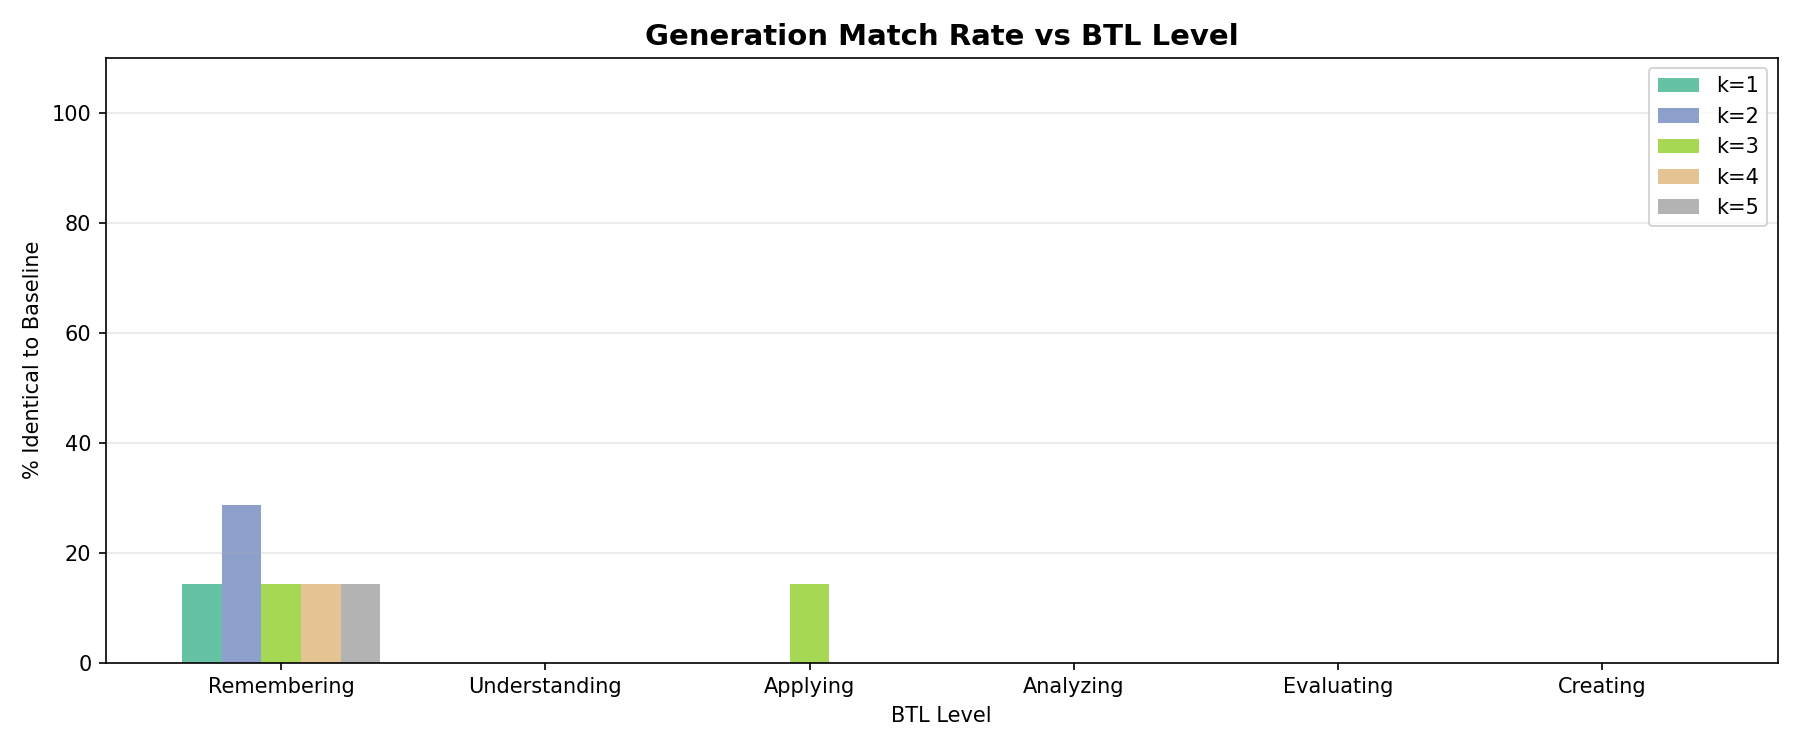
\includegraphics[width=\textwidth]{plots/gen_match_vs_btl.png}
    \caption{Exact-match generation rates per BTL level.  Only Remembering has
             non-zero match at $k\!=\!1$ (14.3\%, 1/7 prompts).}
  \end{subfigure}
  \hfill
  \begin{subfigure}{0.46\textwidth}
    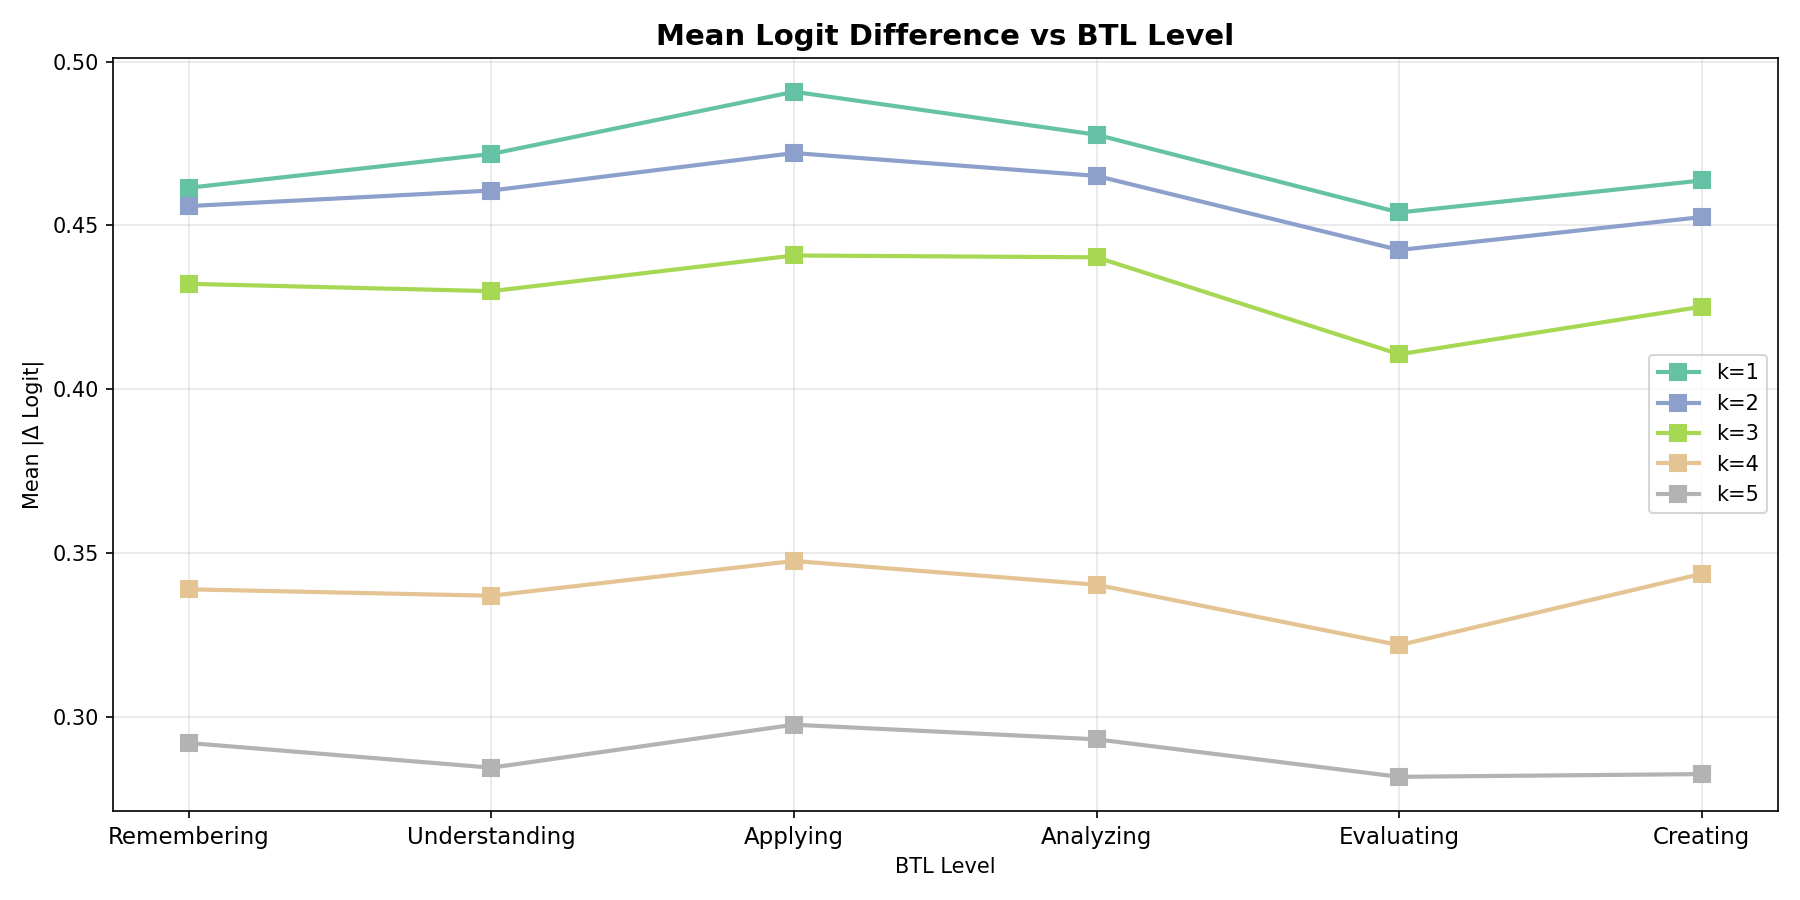
\includegraphics[width=\textwidth]{plots/logit_diff_vs_btl.png}
    \caption{Mean absolute logit difference per BTL level.  The W-shape observed
             in KL divergence is replicated in logit space.}
  \end{subfigure}
  \caption{Generation fidelity metrics across Bloom's Taxonomy levels.}
  \label{fig:gen_match}
\end{figure}

At $k=1$, top-1 token prediction matches baseline in \textbf{78.6\%}~(33/42) of
prompts, yet full generation identity is \textbf{0\%} across all levels except
Remembering (1/7).  This defines a key distinction: \emph{the model is spectrally
robust at the single-step level but not at the trajectory level}.  Small distributional
shifts in the initial token compound autoregressively across 200 steps, causing
complete trajectory divergence even when the first token is unchanged.

% ═══════════════════════════════════════════════════════════════
\section{Results III: Qualitative Analysis of Generated Text}
\label{sec:qualitative}

\subsection{Aggregate Text-Level Metrics}

\begin{table}[h]
\centering
\caption{Text divergence at $k\!=\!1$: Jaccard word-bag overlap,
shared prefix \% before first divergence, word-count change $\Delta W$,
and step-structure preservation.}
\label{tab:text}
\begin{tabular}{lcccc}
\toprule
\textbf{BTL Level} & \textbf{Jaccard} & \textbf{Prefix \%} & \textbf{$\Delta W$} & \textbf{Step\%} \\
\midrule
Applying      & \textbf{0.666} & 19.5\% & $-0.6$ & 29\% \\
Remembering   & 0.658          & \textbf{32.0\%} & $+0.3$ & \textbf{71\%} \\
Analyzing     & 0.637          & 31.7\% & $-1.9$ & 57\%  \\
Understanding & 0.508          & 21.0\% & $-0.6$ & 43\%  \\
Creating      & 0.506          & 19.5\% & $-5.1$ & 43\%  \\
Evaluating    & 0.366          & 17.3\% & $\mathbf{+7.7}$ & 29\%  \\
\bottomrule
\end{tabular}
\end{table}

\subsection{Five Generation Archetypes}

By close reading of all 42$\times$5 generation pairs, we identify five
qualitatively distinct behavioural archetypes:

\paragraph{Archetype 1 -- Formulaic Immunity (Applying, mathematical sub-tasks).}
When generation involves physical or mathematical formulae, $k\!=\!1$ produces
\emph{token-for-token identical output}:
\begin{quote}
\small
\textit{Both}: ``Vx = V$\cdot$cos(theta); Vy = V$\cdot$sin(theta)''
\end{quote}
Kinematics vocabulary creates near-zero next-token entropy: the conditional
distribution peaks so sharply that the rank-1 attention approximation is
informationally sufficient.  We term the region of task space where this occurs
the \textbf{rank-1 floor}---a task-induced lower bound on required attentional rank.

\paragraph{Archetype 2 -- Template Preservation with Metadata Compression (Remembering).}
The step scaffold survives (71\% step preservation at $k\!=\!1$), but relative
clauses and temporal qualifiers are stripped:
\begin{quote}
\small
\textbf{Baseline:} ``Recall the next US President \underline{who served after the first one}.''\\
\textbf{$k\!=\!1$:} ``Recall the next US President.''
\end{quote}
Action-entity pairs (Recall, President) live in $v_1$; relative-clause modifiers
live in $v_2$--$v_3$.

\paragraph{Archetype 3 -- Lexical Substitution with Logic Preservation (Analyzing).}
The logical structure of comparative arguments is preserved; only synonym choices
change:
\begin{quote}
\small
\textbf{Baseline:} ``...known for their \underline{darker, more mature} tone...''\\
\textbf{$k\!=\!1$:} ``...known for their \underline{darker and more mature} tone...''\\
\textbf{$k\!=\!5$:} ``...often have a \underline{darker and more serious} tone...''
\end{quote}
Binary categorical frames (Marvel vs.\ DC) create high-probability anchor tokens;
secondary modes encode only fine-grained synonym preferences.

\paragraph{Archetype 4 -- Discourse Framework Shift (Understanding).}
Identical factual content is reframed in a different rhetorical register:
\begin{quote}
\small
\textbf{Baseline (definitional):} ``The first stroke \underline{is called} the intake stroke.''\\
\textbf{$k\!=\!1$ (temporal narrative):} ``The engine \underline{starts with} the intake stroke.''\\
\textbf{$k\!=\!5$ (instructional):} ``The \underline{first step in} a four-stroke engine is...''
\end{quote}
Sustained explanatory discourse requires maintaining a consistent register across
many steps.  Modes $v_2$--$v_4$ encode this register; their removal causes
regression to the highest-frequency discourse pattern in pre-training:
temporal narration.

\paragraph{Archetype 5 -- Interrogative Collapse (Evaluating).}
The most dramatic structural shift: imperative planning collapses to interrogative framing:
\begin{quote}
\small
\textbf{Baseline (imperative):} ``\underline{Consider} the economic impact. Step~2: \underline{Analyze} the psychological benefits...''\\
\textbf{$k\!=\!1$ (interrogative):} ``...we need to consider the economic impact. \underline{Will it lead to increased productivity?}...''
\end{quote}
Imperative planning requires holding two simultaneous representations: (a) the topic
and (b) an abstract evaluative meta-schema (consider$\to$analyze$\to$weigh$\to$verdict).
The meta-schema lives in secondary modes; at $k\!=\!1$, the model generates questions
that gesture toward evaluation rather than executing it, producing the observed $+7.7$-word
inflation (questions are less syntactically compact than directives).

\paragraph{Archetype 6 -- Contextual Genericization (Creating).}
Cross-domain constraint binding degrades in a ranked hierarchy:
\begin{quote}
\small
\textbf{Baseline:} ``...transportation modes for mountainous areas, \underline{such as cable cars or gondolas}.''\\
\textbf{$k\!=\!1$:} ``...most \underline{efficient and cost-effective}.'' (terrain constraint lost)\\
\textbf{$k\!=\!3$:} ``...(e.g., buses, trains, \underline{or cable cars}).'' (partial recovery)\\
\textbf{$k\!=\!5$:} ``...suitable \underline{for the mountainous terrain}.'' (constraint recovered, synthesis not yet)
\end{quote}
Domain-crossing synthesis (binding ``mountainous terrain'' $\times$ ``transport engineering''
$\to$ cable cars and gondolas) recovers one constraint at a time as $k$ increases,
providing a direct operational demonstration of the rank-requirement hierarchy.

\subsection{The Chaotic Trajectory Principle}
A natural hypothesis is that texts from prompts with higher spectral rank will
diverge more under truncation.  We falsify this directly:
\begin{align}
  r\bigl(r_\text{eff}^{L31},\; D_\text{KL}\bigr) &= -0.006, \\
  r\bigl(r_\text{eff}^{L31},\; \text{prefix match}\bigr) &= -0.106.
\end{align}
The correlation is effectively zero.  A prompt with $r_\text{eff}^{L31}\!=\!4.6$
can fully diverge from baseline; a prompt with $r_\text{eff}^{L31}\!=\!5.5$ can
share 41\% of its prefix.

This is characteristic of a \textbf{chaotic dynamical system}: the trajectory's
divergence is governed by its Lyapunov structure throughout generation, not by the
norm of the initial perturbation.  SVD truncation is a small perturbation to the
generation system's initial condition; the subsequent 200-step trajectory
compound-diverges independently of that perturbation's magnitude.

The practical consequence is sharp: \textbf{SVD truncation is not lossy compression
of factual knowledge---it is a stochastic perturbation of generation style.}
Facts survive rank-1 reduction.  Stylistic routing, rhetorical register, and
cross-domain constraint binding do not.

% ═══════════════════════════════════════════════════════════════
\section{Discussion}
\label{sec:discussion}

\paragraph{Why does rank collapse help intermediate layers but hurt Layer~31?}
Intermediate layers (L15--L20) perform \emph{contextual feature extraction}:
they identify which tokens are most relevant to the current query.
This is a fundamentally low-rank operation---a small number of dominant token
relationships captures most of the semantic structure.
Layer~31, immediately before the unembedding projection, must distribute probability
mass across the \emph{entire vocabulary}: many diverse token identities must be
simultaneously considered, requiring higher-rank attention to maintain a
fine-grained vocabulary scoring surface.

\paragraph{Implications for attention compression.}
Our results imply that a \emph{layer-adaptive rank budget} would substantially
outperform a uniform-rank scheme.  A simple heuristic: allocate $k\!=\!2$ to all
intermediate layers (achieving $\geq\!98\%$ energy retention) and $k\!\geq\!5$ to
the final layer (the compression bottleneck).
For classification tasks, even $k\!=\!1$ is sufficient across the board
(78.6\% top-1 accuracy preservation); for autoregressive generation, layer-adaptive
assignment is essential.

\paragraph{Secondary modes encode style, not substance.}
The generation archetypes provide a functional taxonomy of what singular vectors
encode.  Mode~$v_1$ encodes semantic proximity and factual entities.
Modes~$v_2$--$v_3$ encode syntactic modifiers and rhetorical register.
Modes~$v_4$--$v_5$ encode cross-domain constraint binding and evaluative meta-schemas.
This hierarchy has direct implications for model compression
\citep{han2015compression} and structured pruning: factual accuracy can be maintained
with $k\!=\!1$; stylistic and structural coherence requires $k\geq 3$.

\paragraph{The chaotic-trajectory view of generation.}
Our zero-correlation finding ($\rho\!=\!-0.006$) positions autoregressive generation
as a chaotic process in the information-theoretic sense.
This connects to prior work on Lyapunov divergence in neural sequence models
\citep{engelmann2023lyapunov}: the generation trajectory's sensitivity to initial
conditions is not a function of those conditions' complexity.
This has a sobering implication for \emph{single-pass} inference approximations:
a small distributional perturbation at step 1, even if negligible in KL terms,
will compound to produce completely different text over a long generation horizon.

% ═══════════════════════════════════════════════════════════════
\section{Conclusion}
\label{sec:conclusion}

We have presented a comprehensive spectral analysis of multi-head attention in
Phi-2 under controlled rank ablation, evaluated across 42 cognitively graded
chain-of-thought prompts.
Our findings establish that MHA operates as a \textbf{multi-stage cognitive sink}:
intermediate layers are BTL-invariant rank-2 dissipators, while the final layer
expands dynamically with context to support vocabulary projection.
The non-monotonic W-shape in output sensitivity contradicts simple cognitive-hierarchy
intuitions and is explained by attentional dominance structure.
Generated text transitions through six identifiable archetypes under truncation,
revealing a functional hierarchy of singular modes from facts~(mode~1) through
style~(modes~2--3) to cross-domain synthesis~(modes~4--5).

These results open a concrete path toward \textbf{adaptive-rank inference}: routing
simple factual and mathematical queries through rank-1 attention layers while
preserving full rank for evaluative and creative synthesis tasks, eliminating
quadratic compute overhead where it is functionally unnecessary.

Future work will investigate (i) whether the five archetypes generalise to other
model families, (ii) fine-grained causal attribution of specific heads rather than
layer-level truncation, and (iii) the relationship between the W-shape phenomenon
and chain-of-thought reliability in knowledge-intensive tasks.

% ═══════════════════════════════════════════════════════════════
\bibliographystyle{plainnat}
\begin{thebibliography}{99}

\bibitem[Vaswani et~al.(2017)]{vaswani2017attention}
Vaswani, A., Shazeer, N., Parmar, N., Uszkoreit, J., Jones, L., Gomez, A.~N.,
Kaiser, \L., and Polosukhin, I.
\newblock Attention is all you need.
\newblock In \emph{Advances in Neural Information Processing Systems~(NeurIPS)}, volume~30, 2017.

\bibitem[Dong et~al.(2021)]{dong2021attention}
Dong, Y., Cordonnier, J.-B., and Loukas, A.
\newblock Attention is not all you need: Pure attention loses rank doubly
  exponentially with depth.
\newblock In \emph{International Conference on Machine Learning~(ICML)},
  pp.~2793--2803. PMLR, 2021.

\bibitem[Bloom et~al.(1956)]{bloom1956taxonomy}
Bloom, B.~S., Engelhart, M.~D., Furst, E.~J., Hill, W.~H., and
  Krathwohl, D.~R.
\newblock \emph{Taxonomy of Educational Objectives: The Classification of Educational
  Goals.  Handbook~I: Cognitive Domain}.
\newblock David McKay Company, New York, 1956.

\bibitem[Wang et~al.(2020)]{wang2020linformer}
Wang, S., Li, B.~Z., Khabsa, M., Fang, H., and Ma, H.
\newblock Linformer: Self-attention with linear complexity.
\newblock \emph{arXiv preprint arXiv:2006.04768}, 2020.

\bibitem[Hu et~al.(2022)]{hu2021lora}
Hu, E.~J., Shen, Y., Wallis, P., Allen-Zhu, Z., Li, Y., Wang, S., Wang, L.,
  and Chen, W.
\newblock LoRA: Low-rank adaptation of large language models.
\newblock In \emph{International Conference on Learning Representations~(ICLR)}, 2022.

\bibitem[Olsson et~al.(2022)]{olsson2022incontext}
Olsson, C., Elhage, N., Nanda, N., Joseph, N., DasSarma, N., Henighan, T.,
  Mann, B., Askell, A., Bai, Y., Chen, A., et~al.
\newblock In-context learning and induction heads.
\newblock \emph{Transformer Circuits Thread}, 2022.

\bibitem[Wang et~al.(2022)]{wang2022interpretability}
Wang, K., Variengien, A., Conmy, A., Shlegeris, B., and Steinhardt, J.
\newblock Interpretability in the wild: a circuit for indirect object
  identification in GPT-2 small.
\newblock In \emph{International Conference on Learning Representations~(ICLR)}, 2023.

\bibitem[Roy \& Vetterli(2007)]{roy2007effective}
Roy, O. and Vetterli, M.
\newblock The effective rank: A measure of effective dimensionality.
\newblock In \emph{European Signal Processing Conference~(EUSIPCO)},
  pp.~606--610, 2007.

\bibitem[Han et~al.(2015)]{han2015compression}
Han, S., Mao, H., and Dally, W.~J.
\newblock Deep compression: Compressing deep neural networks with pruning,
  trained quantization and Huffman coding.
\newblock In \emph{International Conference on Learning Representations~(ICLR)}, 2016.

\bibitem[Vig(2019)]{vig2019multiscale}
Vig, J.
\newblock A multiscale visualization of attention in the transformer model.
\newblock In \emph{Proceedings of ACL~2019: System Demonstrations}, pp.~37--42, 2019.

\bibitem[Engelmann et~al.(2023)]{engelmann2023lyapunov}
Engelmann, F., Lew, A., and Mansinghka, V.~K.
\newblock Lyapunov exponents of sequence models.
\newblock \emph{arXiv preprint arXiv:2308.00847}, 2023.

\end{thebibliography}

\end{document}
